\subsubsection{UC14 - Gestione ordini}
\begin{figure}[h]
	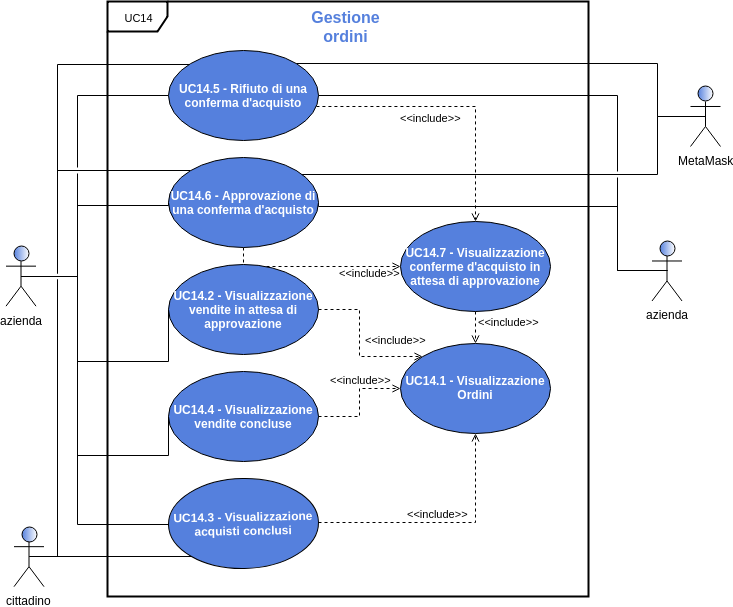
\includegraphics[width=10cm]{res/images/UC14-GestioneOrdini.png}
	\centering
	\caption{UC14 - Gestione ordini}
\end{figure}
\begin{itemize}
	\item \textbf{Attori Primari}: azienda, cittadino;
	\item \textbf{Descrizione}: agli utenti sono messe a disposizione diverse operazione per visualizzare e gestire gli ordini;
	\item \textbf{Scenario principale}: l'utente visualizza e svolge alcune operazioni per gestire gli ordini nei quali è partecipe;
	\item \textbf{Precondizione}: il sistema ha riconosciuto l'utente autenticato come azienda o cittadino e mette a disposizione tutte le pagine necessarie alla visualizzazione e gestione degli ordini;
	\item \textbf{Postcondizione}: l'utente ha visualizzato e/o gestito i propri ordini.
\end{itemize} 
\subsubsection{UC14.1 - Visualizzazione ordini}
\begin{itemize}
	\item \textbf{Attori Primari}: azienda, cittadino;
	\item \textbf{Descrizione}: alle aziende ed ai cittadini sono messe a disposizione diverse operazioni per visualizzare e gestire gli ordini all'interno della piattaforma. Essi comprendono acquisti e vendite (queste solo per le aziende). \`E reso possibile avere un elenco dettagliato di tutti gli ordini, in particolare per ognuno di essi è possibile la visualizzazione:
	\begin{itemize}
		\item della data dell'ordine;
		\item del numero dell'ordine;
		\item dei prodotti inclusi nell'ordine [UC5];
		\item totale IVA;
		\item totale lordo\glo;
		\item indirizzo di spedizione.
	\end{itemize}
	\item \textbf{Scenario principale}: l'utente visualizza i dati relativi ad un ordine;
	\item \textbf{Inclusioni}:
	\begin{itemize}
		\item \textbf{UC5}: visualizzazione dei beni.
	\end{itemize}
	\item \textbf{Precondizione}: il sistema ha riconosciuto l'utente autenticato come azienda o cittadino e mette a disposizione tutte le pagine necessarie alla visualizzazione e gestione degli ordini;
	\item \textbf{Postcondizione}: l'utente ha visualizzato l'elenco dei propri ordini.
\end{itemize} 



\subsubsection{UC14.2 - Visualizzazione acquisti conclusi}
\begin{itemize}
	\item \textbf{Attori Primari}: cittadino, azienda;
	\item \textbf{Descrizione}: l'azienda ha la possibilità di visualizzare gli acquisti conclusi, ovvero effettuati ed approvati. Oltre ai dati relativi all'ordine sono visualizzate le seguenti informazioni:
	\item \textbf{Scenario principale}: l'utente visualizza la lista degli acquisti conclusi. Oltre ai campi relativi agli ordini sono visualizzate le seguenti informazioni:
	\begin{itemize}
		\item data dell'approvazione dell'ordine;
		\item nome dell'azienda-venditrice;
		\item partita IVA dell'azienda venditrice.
	\end{itemize}
	
	\item \textbf{Inclusioni}:
	\begin{itemize}
		\item \textbf{UC14.1}: Visualizzazione degli ordini.
	\end{itemize}
	\item \textbf{Precondizione}: l'utente sta visitando la pagina contenente la lista degli acquisti conclusi;
	\item \textbf{Postcondizione}: l'utente visualizza la lista degli acquisti conclusi.
\end{itemize}

\subsubsection{UC14.3 - Visualizzazione vendite concluse}
\begin{itemize}
	\item \textbf{Attori Primari}: azienda;
	\item \textbf{Descrizione}: l'azienda ha la possibilità di visualizzare le vendite effettuate ed approvate. Oltre ai dati relative all'ordine sono visualizzare le seguenti informazioni:
		\begin{itemize}
		\item data dell'approvazione;
		\item informazioni riguardanti il cliente:
		\begin{itemize}
			\item nel caso il cliente sia un \textbf{cittadino}:
			\begin{itemize}
				
				\item nome utente;
				\item cognome utente.
			\end{itemize}
			\item nel caso il cliente sia un'\textbf{azienda}:
			\begin{itemize}
				
				\item nome azienda-cliente;
				\item partita IVA dell'azienda-cliente.
			\end{itemize}
		\end{itemize}
		
	\end{itemize}
	\item \textbf{Scenario principale}:  l'utente visualizza le vendite concluse, con alcuni dati relativi al cliente; 
	\item \textbf{Inclusioni}:
	\begin{itemize}
		\item \textbf{UC14.1}: visualizzazione degli ordini.
	\end{itemize}
	\item \textbf{Precondizione}: il sistema ha riconosciuto l'utente autenticato come azienda e questo si trova nella pagina dedicata alla visualizzazione delle vendite concluse;
	\item \textbf{Postcondizione}: l'utente visualizza la lista delle vendite concluse.
\end{itemize}


\subsubsection{UC14.4 - Rifiuto di una conferma d'acquisto}
\begin{itemize}
	\item \textbf{Attori Primari}: azienda, cittadino;
	\item \textbf{Attori Secondari}: MetaMask\glo, azienda;
	\item \textbf{Descrizione}: le aziende ed i cittadini possono rifiutare una conferma d'acquisto\glo, ad esempio se notano che i dati inviatogli non corrispondono all'ordine effettuato o le aliquote IVA imposte risultano errate. Per effettuare l'operazione verrà utilizzato MetaMask\glo;
	\item \textbf{Scenario principale}: l'utente visualizza una conferma d'acquisto\glosp che necessita di approvazione e decide di rifiutarla;
	\item \textbf{Inclusioni}: 
	\begin{itemize}
		\item \textbf{UC14.6}: visualizzazione delle conferme d'acquisto 
		relative agli acquisti in attesa di approvazione.
	\end{itemize}
	\item \textbf{Precondizione}: il sistema ha riconosciuto l'utente autenticato come cittadino o azienda ed ha mostrato la lista delle proposte d'acquisto\glosp che necessitano di conferma;
	\item \textbf{Postcondizione}: l'azienda ha rifiutato la proposta 
	d'acquisto\glo. La proposta non sarà più presente nella lista di attesa per 
	la conferma. Il sistema ritorna l'ammontare trattenuto per l'ordine 
	all'acquirente.
\end{itemize}
\subsubsection{UC14.5 - Approvazione di una conferma di acquisto}
\begin{itemize}
	\item \textbf{Attori Primari}: azienda, cittadino;
	\item \textbf{Attori Secondari}: MetaMask\glo, azienda;
	\item \textbf{Descrizione}: l'azienda accetta la proposta d'acquisto\glosp ricevuta;
	\item \textbf{Scenario principale}: l'azienda/cittadino decide di approvare una proposta d'acquisto\glosp da parte di un venditore;
	\item \textbf{Scenario alternativo}: l'azienda/cittadino non ha né confermato né approvato la conferma d'acquisto entro la data ultima per l'approvazione;
		\item \textbf{Inclusioni}: 
	\begin{itemize}
		\item \textbf{UC14.6}:  visualizzazione delle conferme d'ordine\glosp 
		relative agli acquisti in attesa di approvazione.
	\end{itemize}
	\item \textbf{Precondizione}: 
	\begin{enumerate}[label=\alph*.]
		\item il sistema ha riconosciuto l'utente autenticato come azienda o cittadino, e questo ha premuto il bottone per l'approvare una richiesta d'acquisto;
		\item è stata superata la data ultima per il rifiuto della conferma d'ordine\glo.
	\end{enumerate}
	\item \textbf{Postcondizione}: il suddetto ordine risulta approvato. Il meccanismo di escrow\glosp implementato nel sistema rende disponibile la fattura dell'ordine nella pagina dedicata dell'account del cliente. Inoltre l'ammontare relativo all'ordine attualmente trattenuto dal sistema viene versato all'azienda-venditrice.
\end{itemize}


\subsubsection{UC14.6 - Visualizzazione conferme d'acquisto in attesa di 
approvazione}
\begin{itemize}
	\item \textbf{Attori Primari}: azienda, cittadino;
	\item \textbf{Descrizione}: l'azienda/cittadino può visualizzare le conferme d'acquisto\glosp che necessitano di approvazione. Esse sono relative agli acquisti che ha effettuato ma non ancora approvato. Le conferme d'acquisto permettono di visualizzare gli stessi dati relativi ad un ordine, ma ogni prodotto visualizzato ha i seguenti dati aggiuntivi:
	\begin{itemize}
		\item prezzo netto del prodotto acquistato;	
		\item aliquota IVA applicata al prodotto.
	\end{itemize}
	\item \textbf{Scenario principale}: l'utente visualizza la lista delle 
	conferme d'acquisto\glosp che necessitano di conferma. Per ognuna di esse 
	ha la possibilità di confermare la proposta [UC14.5] o di rifiutarla 
	[UC14.4];
	\item \textbf{Inclusioni}:
	\begin{itemize}
		\item \textbf{UC14.1}: Visualizzazione degli ordini;
	\end{itemize}
	\item \textbf{Precondizione}: il sistema ha riconosciuto l'utente autenticato come azienda o cittadino, e questo si trova nella pagina dedicata alla visualizzazione delle conferme d'acquisto\glosp che necessitano di approvazione;
	\item \textbf{Postcondizione}: l'utente visualizza la lista delle conferme d'ordine\glosp che necessitano di approvazione.
\end{itemize}





